%%Chapter - Split into separate file if too large
\chapter{Desserts}

%%Start recipe
\newrecipe{Ricotta Custards with Macerated Strawberries}{}

%% \begin{figure}[h!]
%% \centering
%% \includegraphics[scale=0.75]{./img/image.jpg}
%% \end{figure}

\section*{Ingredients}
\begin{ingredients-list}
	\item 300 g fresh ricotta
	\item \sfrac{1}{2} cup (125ml) thickened cream
	\item 1 egg, plus 2 extra yolks
	\item \sfrac{1}{3} cup (4 tbs) honey
	\item 2 tbs roughly chopped almonds
\end{ingredients-list}
Macerated strawberries:
\begin{ingredients-list}
	\item 250g strawberries, hulled, halved if Large
	\item 1 tbs caster sugar
	\item \sfrac{1}{4} tsp finely grated orange zest
	\item 1 tbs balsamic vinegar
\end{ingredients-list}

\section*{Directions}
\begin{enumerate}
	\item Preheat the oven to 150\textcelsius.
	\item  For the macerated strawberries, place in a bowl and sprinkle with sugar
	\item Combine the orange zest and balsamic vinegar. Pour over the strawberries and toss to coat. Set aside.
	\item Firmly press ricotta through a coarse sieve into a bowl using a spatula or the back of a spoon.
		Scrape the underside of the sieve frequently. Gently fold in the cream and set aside.
	\item Place egg, egg yolks and honey in a bowl and whisk until honey is incorporated and mixtureis light and fluffy.
			Fold the egg mixture gently into the ricotta mixture.
	\item Place four \sfrac{1}{2}-cup (125ml) ramekins or ovenproof ceramic cups in a baking dish.
			Fill each ramekin with the ricotta mixture and top with the almonds.
			Fill the baking dish with enough boiling water to come halfway up the sides of the ramekins, then carefully place the baking dish in the oven.
			Bake for about 45 minutes or until the mixture is just set. Cool slightly then chill custards for 1 hour or until ready to serve.
	\item Serve the chilled ricotta custards with the macerated strawberries.
\end{enumerate}

%%End recipe


%%Start Recipe
\newrecipe{Sticky Date Pudding with Butterscotch Sauce and Almond Praline}{}

\section*{Ingredients}
\begin{ingredients-list}
	\item 180g dates, pitted and roughly chopped
	\item 1\sfrac{1}{4} cups (310ml) water
	\item \sfrac{1}{2} tsp bicarbonate of soda
	\item \sfrac{3}{4} cup (165g) firmly packed brown sugar
	\item 60g butter, softened chopped
	\item 2eggs
	\item 1 cup (150g) self-raising flour
\end{ingredients-list}
Almond praline
\begin{ingredients-list}
	\item \sfrac{1}{2} cup (110g) caster sugar
	\item \sfrac{1}{4} cup (35g) slivered almonds Butterscotch sauce
	\item 50g butter
	\item 1 cup (220g) brown sugar
	\item 1 cup (250ml) cream
	\item 1 tsp vanilla extract
\end{ingredients-list}

\section*{Directions}
\begin{enumerate}
	\item Preheat oven to 180 \textcelsius\ (160 \textcelsius\            fan·forced). Lightly grease eight (\sfrac{1}{2} cup capacity) metal dariole moulds.
	\item Place dates and water in a saucepan and bring to the boil over a high heat. Remove from the heat.
		Add bicarbonate of soda, stir until dates start to break down, set aside to cool, stirring occasionally.
	\item Beat butter and sugar in a bowl using a hand beater, gradually add eggs one at a time, beat until light and fluffy.
	\item Add date mixture, stir to combine. Carefully fold through sifted flour, divide mixture evenly between the eight moulds, until \sfrac{2}{3} full.
	\item Place moulds in a baking tray, carefully pour water in tray until it comes up \sfrac{1}{3} of the side of the moulds.
		Bake in oven for 40 minutes or until golden and skewer comes out clean.
	\item Meanwhile, for the almond praline, combine sugar and 2 tablespoons water in a saucepan over medium heat and cook caramel without stirring,
		swirling pan, until deep golden. Scatter almonds onto a baking paper·lined oven tray, pour over caramel and cool until set. Break praline into pieces.
	\item For the butterscotch sauce, combine butter, sugar, cream and vanilla in small saucepan over low heat until butter melts and sugar dissolves.
		Bring sauce to the boil, reduce heat and cook for 5·6 minutes or until sauce thickens slightly.
	\item To serve, invert the hot pudding onto a serving plate, top with butterscotch sauce and shards of praline.
\end{enumerate}
%%End Recipe

%%Start recipe
\newrecipe{Baked Strawberry Cheesecake}{http://www.kraftrecipes.com/recipes/philadelphia-classic-cheesecake-52544.aspx}

\section*{Ingredients}
\begin{ingredients-list}
	\item 1\sfrac{1}{2} cups scallywag/golliwog biscuit Crumbs
	\item 3 Tbsp. sugar
	\item \sfrac{1}{3} cup butter or margarine, melted
	\item 4 packs (250g each) PHILADELPHIA Cream Cheese/or Woolworths Homebrand, softened
	\item 1 cup sugar
	\item 1 tsp. vanilla
	\item 4eggs
\end{ingredients-list}

Stawberry Topping
\begin{ingredients-list}
	\item 2 punnets (250g each) of strawberries
	\item 1 tablespoon cornstarch
	\item 2-3 tablespoon water
\end{ingredients-list}

\section*{Directions}
\begin{enumerate}
	\item Pre-heat oven to 160 \textcelsius
	\item MIX biscuit crumbs, 3 tbsp. sugar and butter; press onto bottom of 23cm springform pan.
	\item BEAT cream cheese, 1 cup sugar and vanilla with mixer until well blended.
		Add eggs, 1 at a time, mixing on low speed after each just until blended. Pour over crust.
	\item BAKE 55 min. or until centre is almost set.
	\item Cool in the oven with the door open to avoid splitting.
	\item Loosen cake from rim of pan. Refrigerate 4 hours.
\end{enumerate}
	Strawberry Topping
\begin{enumerate}
	\item Cut the strawberries into smaller pieces (Reserve 1⁄4 - 1⁄2 for decorating)and place into a saucepan on the stovetop.
		Bring to a boil, stirring continuously for about 10 minutes. Add a small amount of water to start if needed.
	\item Add 1 cup of sugar to the mixture and stir until the sugar has melted.
	\item Mix the cornstarch with 2-3 tablespoons of water or until runny.
		Add the cornstarch to the strawberries, stirring continuously as the mixture boils for another 5 minutes.
		Remove from the stovetop.
	\item Allow the strawberry sauce to cool (place into an ice bath for faster cooling) and then blend	it in a blender until smooth.
\end{enumerate}

%%Start recipe
\newrecipe{Pear and Almond Upside Down Cake}{http://www.taste.com.au/recipes/4905/pear+almond+upside+down+cake}

\bigskip
\section*{Ingredients}

\begin{ingredients-list}
	\item 180g brown sugar
	\item 270g unsalted butter, softened
		\begin{textblock*}{8cm}(7.5cm,-1.3cm) % {block width} (coords)
			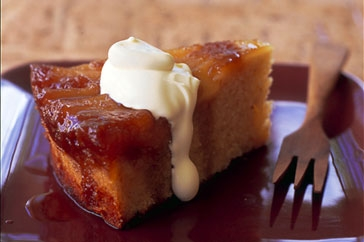
\includegraphics[scale=0.65]{./img/pear_almond.jpg}
		\end{textblock*}
	\item 300g caster sugar
	\item 3 eggs
	\item 1 \sfrac{2}{3} cups (250g) plain flour
	\item 1 \sfrac{1}{2} tsp baking powder
	\item 1 tsp ground cinnamon
	\item \sfrac{1}{2} tsp ground nutmeg
	\item 80g almond meal
	\item 1 cup (250ml) buttermilk
	\item 4 ripe pears (such as beurre bosc), peeled, cored, cut into 2cm-thick slices
	\item Thick cream, to serve 
\end{ingredients-list}

\section*{Directions}
\begin{enumerate}
	\item Preheat oven to 180°C (not fan-forced).
	\item Grease and line base of a 26cm cake pan with baking paper. Sprinkle brown sugar over base.
			Melt 100g butter and pour over brown sugar. Top with overlapping pear slices.
			Place remaining butter and caster sugar in bowl of electric mixer, beat for 5 minutes until light and fluffy.
	\item Add eggs one at a time, beating well after each addition. Sift together flour, baking powder and spices, fold into egg mixture with almond meal.
	\item Stir in buttermilk, then mix to form a smooth batter. Carefully spread over pears.
	\item Place pan on a baking tray, cook for 1 hour and 20 minutes.
	\item Cover loosely with foil if cake begins to brown too quickly. Remove and cool for 30 minutes. Run a knife around sides of pan and carefully invert onto a plate.
	\item Serve with thick cream.
\end{enumerate}
%%End recipe

%%Start recipe
\newrecipe{Blueberry Boy Bait}{http://smittenkitchen.com/blog/2009/07/blueberry-boy-bait/}

\bigskip
\section*{Ingredients}

\begin{ingredients-list}
	\item 2 cups plus 1 teaspoon all-purpose flour
	\item 1 tablespoon baking powder
		\begin{textblock*}{8cm}(8.6cm,-1.3cm) % {block width} (coords)
			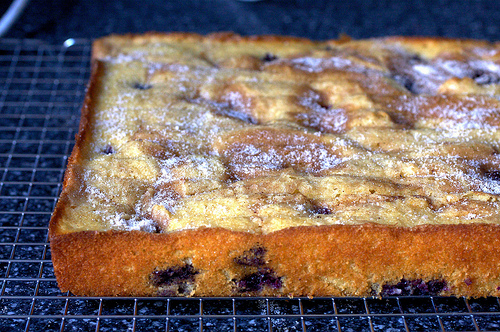
\includegraphics[scale=0.43]{./img/blueberry-boy-bait.jpg}
		\end{textblock*}
	\item 1 teaspoon table salt
	\item 250g unsalted butter (2 sticks), softened
	\item \sfrac{3}{4} cup packed light brown sugar
	\item \sfrac{1}{2} cup granulated sugar
	\item 3 large eggs
	\item 1 cup whole milk
\item \sfrac{1}{2} cup blueberries, fresh or frozen
\end{ingredients-list}

Topping
\begin{ingredients-list}
	\item \sfrac{1}{2} cup blueberries, fresh or frozen (do not defrost)
	\item \sfrac{1}{4} cup granulated sugar
	\item \sfrac{1}/{2} teaspoon ground cinnamon
\end{ingredients-list}

\section*{Directions}
\begin{enumerate}
	\item Preheat oven to 180 \textcelsius\ (170 \textcelsius\  fan-forced).
	\item Grease and 13 x 9 inch baking pan
	\item Whisk two cups flour, baking powder, and salt together in medium bowl.
		With electric mixer, beat butter and sugars on medium-high speed until fluffy, about two minutes. 
	\item Add eggs, one at a time, beating until just incorporated and scraping down bowl.
	\item Reduce speed to medium and beat in one-third of flour mixture until incorporated; beat in half of milk.
	\item Beat in half of remaining flour mixture, then remaining milk, and finally remaining flour mixture.
	\item Toss blueberries with remaining one teaspoon flour. Using rubber spatula, gently fold in blueberries.
		Spread batter into prepared pan.
	\item Scatter blueberries over top of batter.
	\item Stir together sugar and cinnamon and sprinkle over batter.
	\item Bake 45 to 50 minutes or until a toothpick inserted into centre of cake comes out clean.
	\item Cool in pan for 20 minutes then turn out and place on a serving platter.
\end{enumerate}
%%End recipe

%%Start recipe
\newrecipe{Raspberry \& Orange Upside-Down Cake}{http://www.taste.com.au/recipes/22766/raspberry+orange+upside+down+cake}

\bigskip
\section*{Ingredients}

\begin{ingredients-list}
	\item Melted butter, to grease
		\begin{textblock*}{8cm}(8.0cm,-0.8cm) % {block width} (coords)
			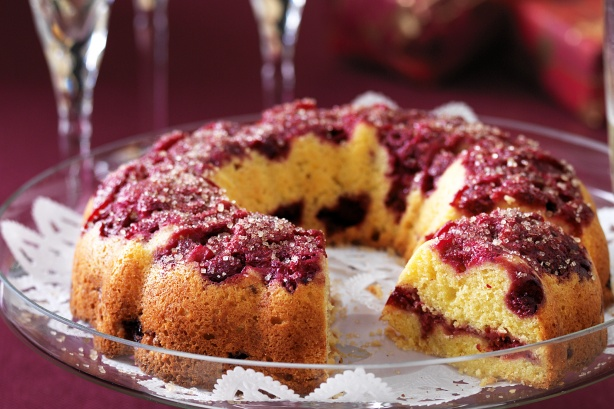
\includegraphics[scale=0.38]{./img/raspberry_orange.jpg}
		\end{textblock*}
	\item 175g butter, chopped, room temp.
	\item 155g (\sfrac{3}{4} cup) caster sugar
	\item 2 tsp finely grated orange rind
	\item 3 eggs
	\item 150g (1 cup) self-raising flour, sifted
	\item 75g (\sfrac{1}{2} cup) plain flour, sifted
	\item 100g almond meal
	\item 80ml (\sfrac{1}{3} cup) fresh orange juice
	\item 300g frozen raspberries
	\item 3 tsp demerara sugar
	\item Double or whipped cream, to serve 
\end{ingredients-list}

\section*{Directions}
\begin{enumerate}
	\item Preheat oven to 180 \textcelsius . Brush a 24cm (top measurement) fluted non-stick ring pan with melted butter to grease.
		Line the base with non-stick baking paper.
	\item Use an electric beater to beat the butter, caster sugar and orange rind in a large bowl until pale and creamy.
		Add the eggs, 1 at a time, beating well after each addition. Fold in the combined flour, almond meal and orange juice.
	\item Arrange half the raspberries in the base of the prepared pan. Top with half the cake mixture. Repeat with remaining raspberries and mixture.
		Tap on the benchtop to settle. Smooth the surface. Bake for 50-55 minutes or until a skewer inserted into the centre comes out clean.
		Set aside for 10 minutes to cool.
	\item Run a flat-bladed knife carefully around the inside edge of the pan. Turn the cake onto a cake stand or serving platter.
	\item Sprinkle with demerara sugar. Slice and serve with cream.

\end{enumerate}
%%End recipe


%%Start recipe
\newrecipe{Lemon Syrup Cake}{}

\bigskip
\section*{Ingredients}

\begin{ingredients-list}
	\item 125g butter,softened.
	\item 1\sfrac{1}{2} cup caster sugar
	\item 1 large lemon, rind finely grated, juiced
	\item 2 eggs
	\item 1\sfrac{1}{2} cup  self-raising flour, sifted
	\item \sfrac{1}{2} cup milk
\end{ingredients-list}

\section*{Directions}
\begin{enumerate}
	\item Preheat oven to 180 \textcelsius . Grease and line a 6 cm deep, 19 x10 cm base loaf pan.
	\item Use an electric beater to beat the butter, 1 cup of caster sugar and lemon rind in a large bowl until pale and creamy.
		Add the eggs, 1 at a time, beating well after each addition.
	\item Add half the flour and half the milk and stir gently to combine. Fold in the remaining flour and milk.
	\item Spoon mixture into loaf pan and bake for 45-50 minutes.
	\item Combine remaining sugar and \sfrac{1}{3} cup of lemon juice and bring to the boil.
	\item Pour over hot loaf while still in pan.  Stand in pan until cooled.

\end{enumerate}
%%End recipe
%%End Chapter